\chapter{Response Meaurement with Single Hadrons}

\newcommand*{\pL}{\ensuremath{\Lambda}\xspace}
\newcommand*{\pLB}{\ensuremath{\bar{\Lambda}}\xspace}
\newcommand*{\pKS}{\ensuremath{K_\text{S}^{0}}\xspace}
\newcommand*{\pKL}{\ensuremath{K_L}\xspace}
\newcommand*{\pip}{\ensuremath{\pi^+}\xspace}
\newcommand*{\pim}{\ensuremath{\pi^-}\xspace}
\newcommand*{\piz}{\ensuremath{\pi^0}\xspace}
\newcommand*{\ep}{\ensuremath{E/p}\xspace}
\newcommand*{\epav}{\ensuremath{\langle E/p \rangle}\xspace}
\newcommand*{\epcor}{\ensuremath{\langle E/p \rangle_{\mathrm{COR}}}\xspace}
\newcommand*{\epbg}{\ensuremath{\langle E/p \rangle_{\mathrm{BG}}}\xspace}
\newcommand*{\Ea}{\ensuremath{E_a}\xspace}
\newcommand*{\QGSP}{\texttt{QGSP\_BERT}\xspace}
\newcommand*{\FTFP}{\texttt{FTFP\_BERT}\xspace}


\label{ch:singlehadrons}
% --------------------------------------------------------------------------------

\section{Overview and Motivation}

As discussed in Section~\ref{sec:jets}, colored particles produced in collisions hadronize into jets of multiple individual hadrons.
As jets form a major component of many physics analyses at ATLAS, it is crucial to carefully calibrate the measurement of jet energies and to derive an uncertainty on that measurement.
These uncertainties have often been the dominant systematic uncertainty in high-energy analyses at the LHC.

One approach to understanding jet physics in the ATLAS calorimetry is to evaluate the calorimeter response to individual hadrons; measurements of individual hadrons can be used to build up an understanding of the jets that they form.
The redundancy of the momentum provided by the tracking system and the energy provided by the calorimeter provides an opportunity to study calorimeter response using real collisions, as described further in Section~\ref{sec:inclusive}.

A number of interesting factors compromise calorimeter respose, and extracting these separately provides insight into many aspects of jet modelling.
First, many charged hadrons interact with the material of the detector prior to reaching the calorimeters and thus do not deposit any energy.
Comparing this effect in data and simulation is a powerful tool in validating the interactions of particles with the material of the detector as well as the model of the detector geometry in simulation, see Section~\ref{sec:zero_fraction}.
The particles which do reach the calorimeter deposit their energy into individual cells, which are then clustered to measure full energy deposits.
Comparing the response in data to simulated hadrons provides a direct evaluation of several aspects of simulation: noise in the calorimeters, the showering of hadronic particles, and the energy deposited by particles in matter, among others (Section~\ref{sec:response}). 
Additionally, comparing the effect of clustering in data and simulation can indirectly test the simulation's modelling of the shape of hadronic showers, see Section~\ref{sec:clustering}.
These measurements are extended to explore several additional effects, such as the dependence on charge or the individual calorimeter layer in Section~\ref{sec:additional}. 

The above studies all use an inclusive selection of charged particles, which are compromised predominantly of pions, kaons, and (anti)protons.
It is also interesting to measure the particle types separately to evaluate the simulated interactions of each particle, particularly at low energies where differences between species are very relevant.
Pions and (anti)protons can be identified through decays of long-lived particles, in particular $\Lambda$, $\overline{\Lambda}$, and $K_{S}^{0}$, and then used to measure response as described above.
This is discussed in detail in Section~\ref{sec:identified}.

Together, these measurements in data provide a thorough understanding of the way hadrons interact with the ATLAS detector and can be used to build up a description of jets, as seen in Chapter~\ref{ch:jes}.
The results in this chapter use data collected at 7 and 8 \TeV collected in 2010 and 2012, respectively.
Both are included as the calorimeter was repaired and recalibrated between those two data-taking periods.
Both sets of data are compared to an updated simulation that includes new physics models provided by \texttt{Geant4}~\cite{GEANT4} and improvements in the detector description~\cite{PERF-2011-08,PERF-2013-05}.
These results can be compared to a similar measurement performed in 2009 and 2010~\cite{PERF-2011-05}, which used the previous version of the simulation framework~\cite{SOFT-2010-01}.

% ----------------------------------------
\section{Dataset and Simulation}

\subsection{Data Samples}
The two datasets used in this chapter are taken from dedicated low-pileup runs where the fraction of events with multiple interactions was negligable, to facilitate measurement of isolated hadrons.
The 2012 dataset at $\sqrt{s} = 8$ \TeV contains 8 million events and correspons to an integrated luminosity of 0.1 nb\tsup{-1}.
The 2010 dataset at $\sqrt{s} = 7$ \TeV contains 3 million events and corresponds to an integrated luminosity of 3.2 nb\tsup{-1}.
This last dataset was also used in the 2010 results~\cite{PERF-2011-05}, but have since been reanalyzed with an updated detector description of the material and alignment.

\subsection{Simulated Samples}
The two datasets above are compared to simulated single-, double-, and non-diffractive events generated with \texttt{Pythia8}~\cite{PYTHIA8} using the A2 configuration of hadronization~\cite{AU2} and the MSTW 2008 parton-distribution function set~\cite{MSTW,MSTW2}.
The conditions and energies for each run are matched in the two simulations.

To evaluate the interaction of hadrons with detector material, the simulation uses two different collections of hadronic physics models, called physics lists, in \texttt{Geant4 9.4}~\cite{G4hadronics}.
The first, \QGSP, combines the Bertini intra-nuclear cascade~\cite{BERT21,BERT22,BERT23} below 9.9 \GeV, a parametrized proton inelastic model from 9.5 to 25 \GeV~\cite{GHEISHA20}, and a quark-gluon string model above 12 \GeV~\cite{QGS15,QGS16,QGS17,QGS18,QGS19}. 
The second, \FTFP, combines the Bertini intra-nuclear cascade~\cite{BERT21,BERT22,BERT23} below 5 \GeV and the Fritiof model~\cite{FTF24,FTF25,FTF26,FTF27} above 4 \GeV.
In either list, where multiple models overlap, the transition between the two models is ensured to be smooth.

\subsection{Event Selection}
The event selection for this study is minimal, as the only requirement is selecting good-quality events with an isolated track. 
Such events are triggered by requiring at least two hits in the minimum-bias trigger scintillators. 
After trigger, each event is required to have exactly one reconstructed vertex, and that vertex is required to have four or more associated tracks.

The particles which enter into the response measurements are first identified as tracks in the inner detector.
To ensure a reliable momentum measurement, these tracks are required to have at least one hit in the pixel detector, six hits in the SCT, and small longitudinal and transverse impact parameters with respect to the primary vertex~\cite{PERF-2011-05}.
For the majority of the measurements in this chapter, the track is additionally required to have 20 hits in the TRT, which significantly reduces the contribution from tracks which undergo nuclear interaction.
This requirement and its effect is discussed in more detail in Section~\ref{sec:additional_studies}. 
In addition, tracks are rejected if there is another track which extrapolates to the calorimeter within a cone of $\Delta R = \sqrt{(\Delta\phi)^2 + (\Delta\eta)^2} < 0.4$.
This requirement guaruntees that the contamination of energy form nearby charged particled is negligible~\cite{PERF-2011-05}.

% ----------------------------------------

\section{Inclusive Hadron Response}
\label{sec:inclusive}

The calorimeter response is more precisely defined as the ratio of the measured calorimeter energy to the true energy carried by the particle, although this true energy is unkown. 
For charged particles, however, the inner detector provides a very precise measurement of momentum (with uncertainty less than 1\%) that can be used as a proxy for true energy.
The ratio of the energy deposited by the charged particle in the calorimeter, $E$, to its momentum measured in the inner detector $p$, forms the calorimeter response measure called \ep.
Though the distribution of \ep is interesting, two aggregated quantities are more directly useful: \epav, the average of \ep within a given subset of particles, and the zero fraction, the fraction of particles with no associated clusters in the calorimeter.

The calorimeter energy assigned to a track particle is defined using either cells or clusters. 
When clusters are used, they are formed using a 4--2--0 algorithm~\cite{TopoClusters} that begins with seeds requiring at least 4 times the calorimeter average noise. 
The neighboring celss with at least twice that noise threshold are then added to the cluster, and all bounding cells are then added with no requirement. 
This algorithm minimizes noise contributions through its seeding process, and including the additional layers improves the energy resolution~\cite{Speckmayer}.
The cells or clusters are associated to a given track if they fall within a cone of $\Delta R = 0.2$ of the extrapolated position of the track, which includes about 90\% of the energy on average~\cite{PERF-2011-05}.
This construction is illustrated in Figure~\ref{fig:eoverp_cartoon}.

\begin{figure}[htbp]
\centering
\subfloat[]{
  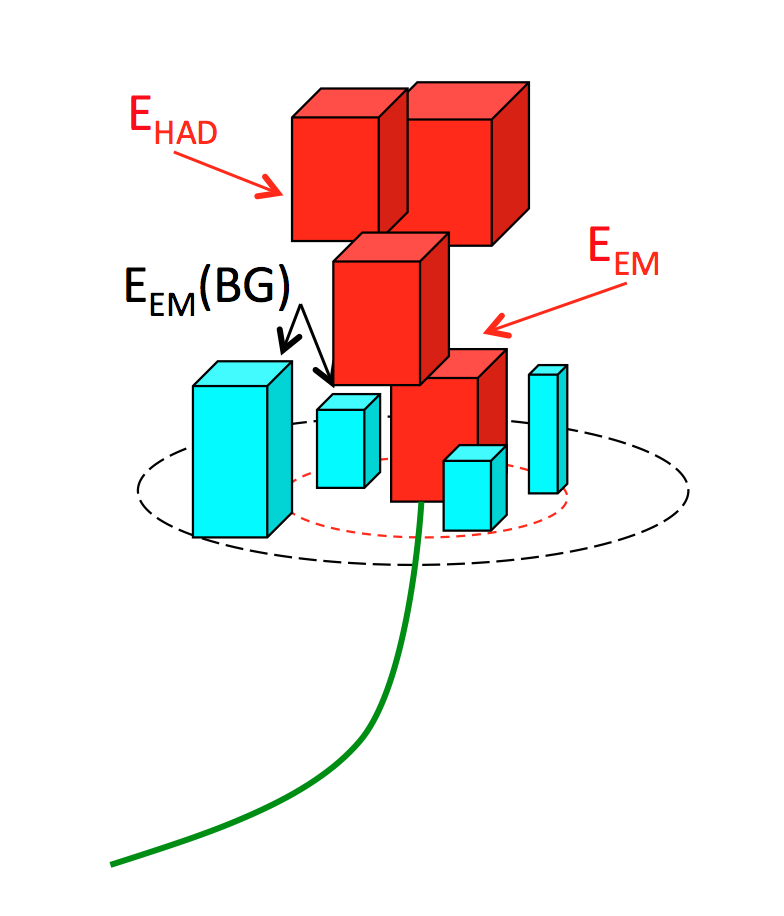
\includegraphics[width=.4\textwidth]{figures/SignalDiagram.png}
}
\subfloat[]{
  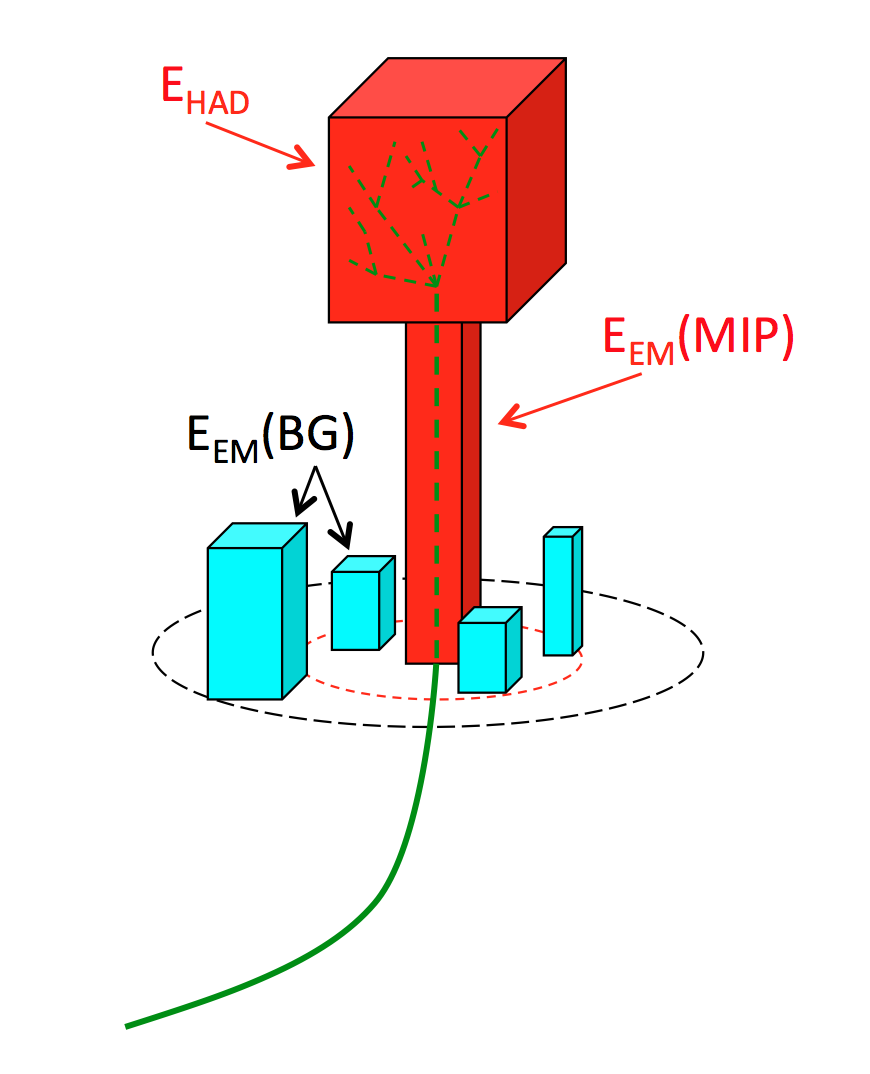
\includegraphics[width=.4\textwidth]{figures/BGDiagram.png}
}
\caption{An illustration (a) of the \ep variable used throughout this paper. The red energy deposits come from the charged particle targeted for measurement, while the blue energy deposits are from nearby neutral particles and must be subtracted. The same diagram (b) for the neutral-background selection, described in Section~\ref{sec:neutral_bg}.}
\label{fig:eoverp_cartoon}
\end{figure}

\subsection{E/p Distribution}

The \ep distributions measured in both data and simulation are shown in Figure~\ref{fig:eoverp} for two example bins of track momentum and for tracks in the central region of the detector. 
These distribution show several important feautres of the \ep observable.
The large content in the bin at $E=0$ comes from tracks that have no associated cluster, as mentioned previously these are due to interactions with detector material prior to reaching the calorimeter or the energy deposit being insufficently large to generate a seed, and are discussed in Section~\ref{sec:zero_fraction}.
The small negative tail comes from similar tracks that do not deposit any energy in the calorimeter but are randomly associated to a noise cluster.
The long positive tail above 1.0 comes from the contribution of neutral particles.
Nearby neutral particles deposit (sometimes large) additional energy in the calorimeter but do not produce tracks in the inner detector and so they cannot be rejected for isolation.
Additionally the peak and mean of the distribution falls below 1.0 because of the loss of energy not found within the cone as well as the non-compensation of the calorimeter.

The data and simulation share the same features, but the high and low tails are significantly different.
The simulated events tend to overstimate the contribution of neutral particle to the long tail, although this effect can be isolated as discussed in Section~\ref{sec:neutral_bg}. 
Additionally, the simulated clusters have less noise on average, although this is a small effect on the overall response.

\begin{figure}[htbp]
\centering
\subfloat[]{
  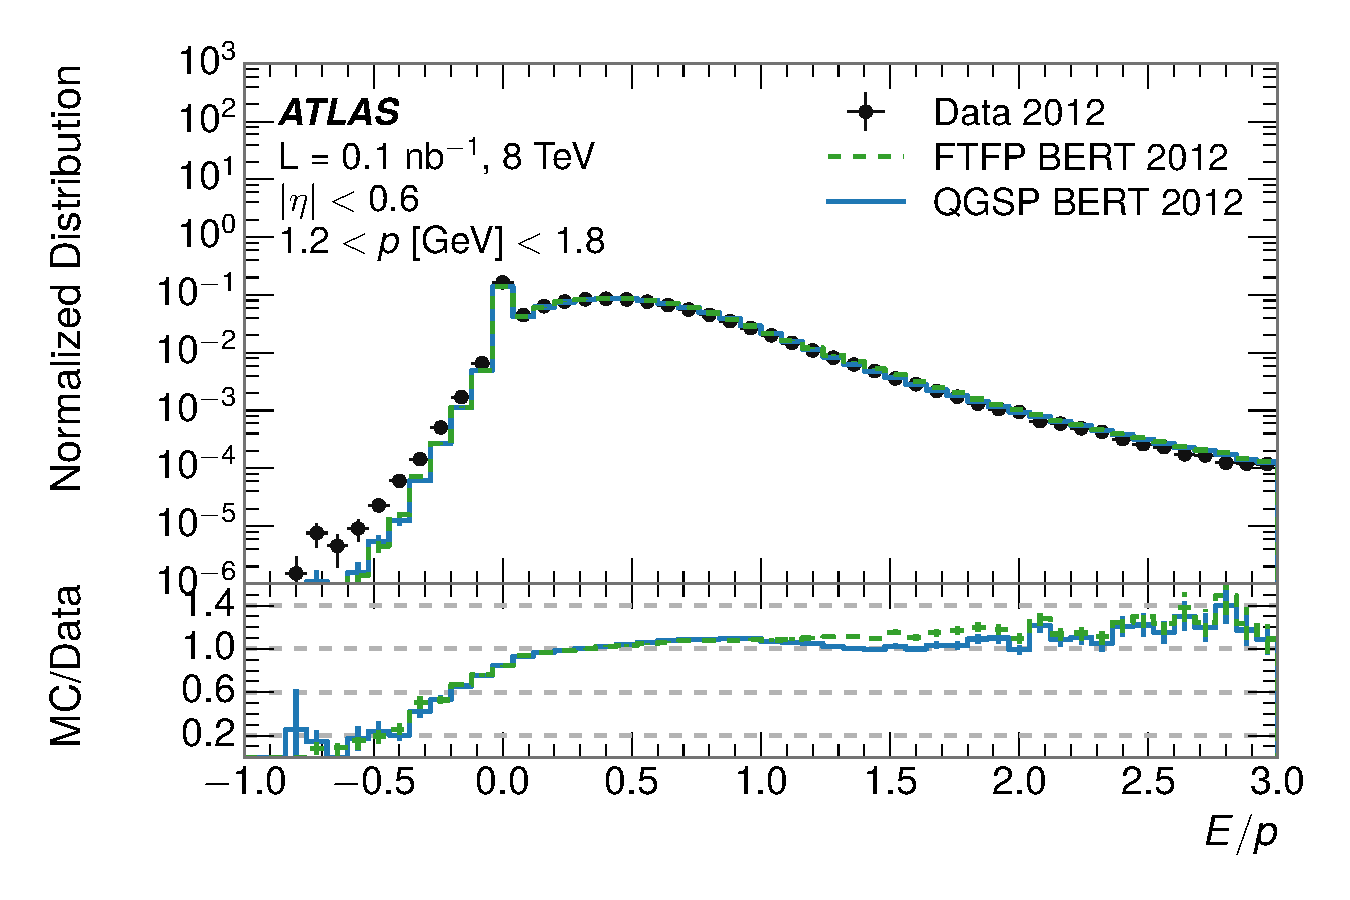
\includegraphics[width=0.48\textwidth]{figures/dvmc12_eoverp_layer01_calib01_eta01_p03_q00_nc00_trt00.pdf}
}
\subfloat[]{
  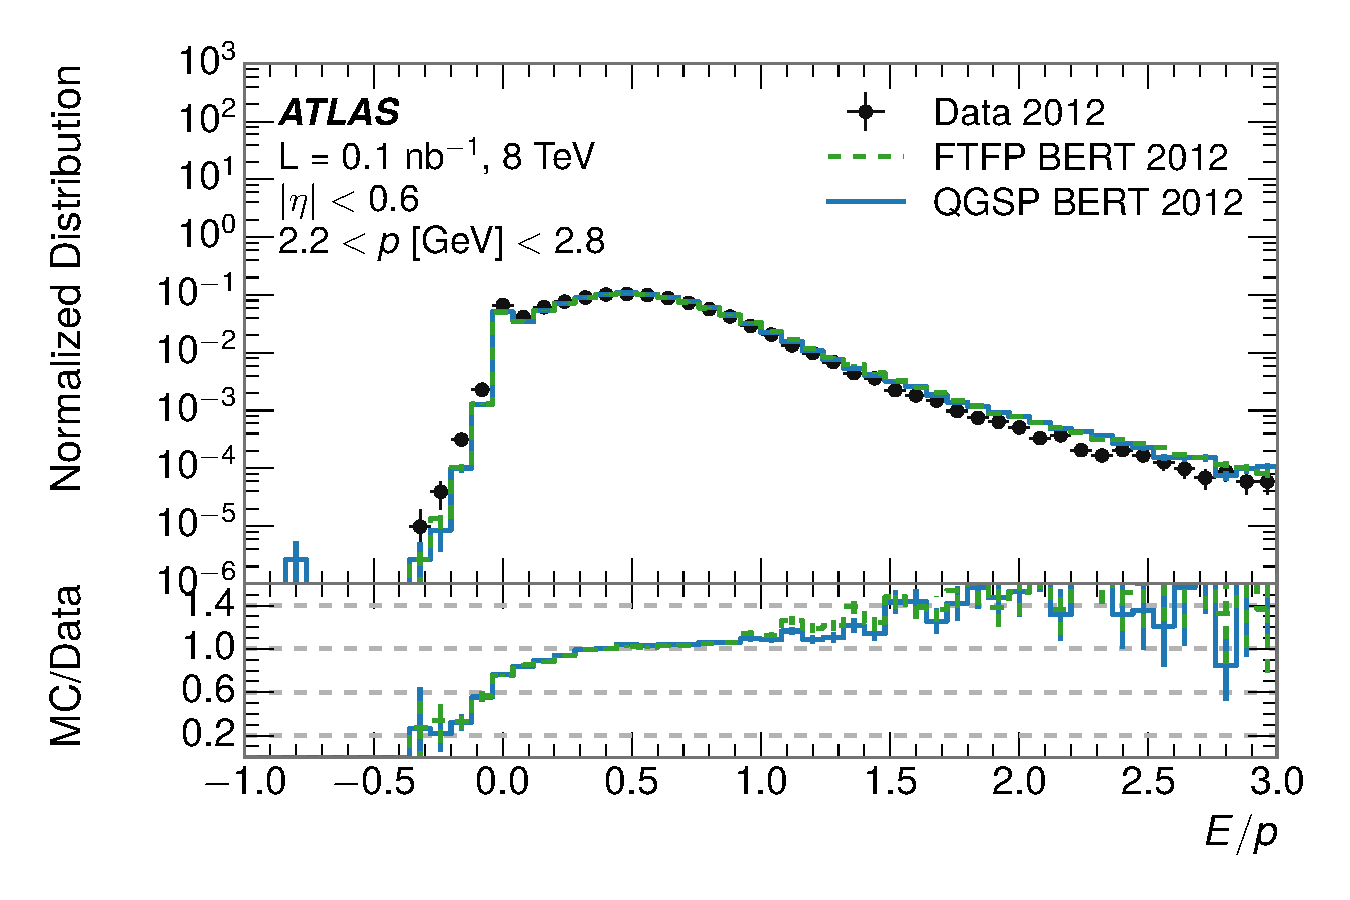
\includegraphics[width=0.48\textwidth]{figures/dvmc12_eoverp_layer01_calib01_eta01_p05_q00_nc00_trt00.pdf}
}
\caption{The \ep distribution and ratio of simulation to data for isolated tracks with (a) $|\eta| < 0.6$ and $1.2 < p /\GeV < 1.8$ and (b) $|\eta| < 0.6$ and $2.2 < p /\GeV < 2.8$.}

\label{fig:eoverp}
\end{figure}

\subsection{Zero Fraction}
\label{sec:zero_fraction}

The fraction of particles with no associated clusters, or similarly those with $E \leq 0$, reflects the modelling of both the detector geometry and hadronic interactions.
The zero fraction is expected to rise as the amount of material a particle traverses increases, while it is expected to decrease as the particle energy increases.
This dependence can be seen in Figure~\ref{fig:zerofracincl}, where the zero fraction in data and simulation is shown as a function of momentum and the amount of material measured in interaction lengths.
The trends are similar between the 2010 and 2012 measurements.
The zero fraction decreases with energy as expected.
The amount of material in the detector increases with $\eta$, which provides a distribution of interaction lengths.
As the data and simulation have significant disagreement in the zero fraction over a number of interaction lengths, the difference must be primarily from the modelling of hadronic interactions.

There is also a noticeable difference between positive at negative tracks at low momentum, which reflects the difference in response between protons and antiprotons.
Antiprotons have significant model differences in the two physics lists, \QGSP and \FTFP, and this is evident in the lowest momentum bin of the data to simulation ratio.
This difference is explored further in Section~\ref{sec:identified}.


\begin{figure}[htbp]
\centering
\subfloat[]{
  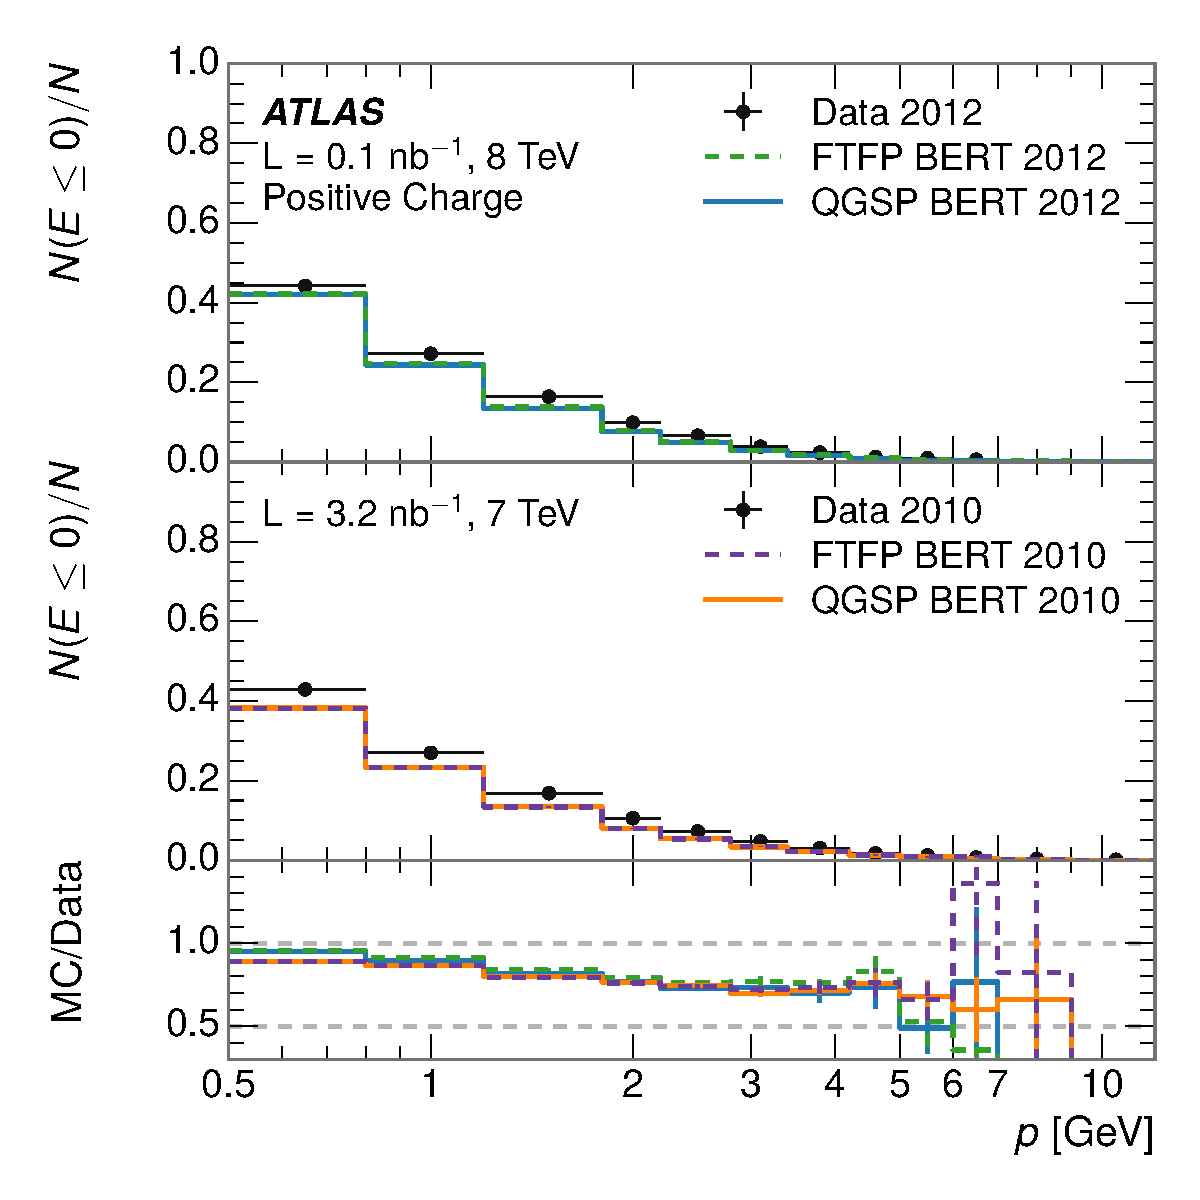
\includegraphics[width=0.48\textwidth]{figures/dvmc_ezero_layer01_calib01_eta01_q02_nc00_trt00.pdf}
}
~
\subfloat[]{
  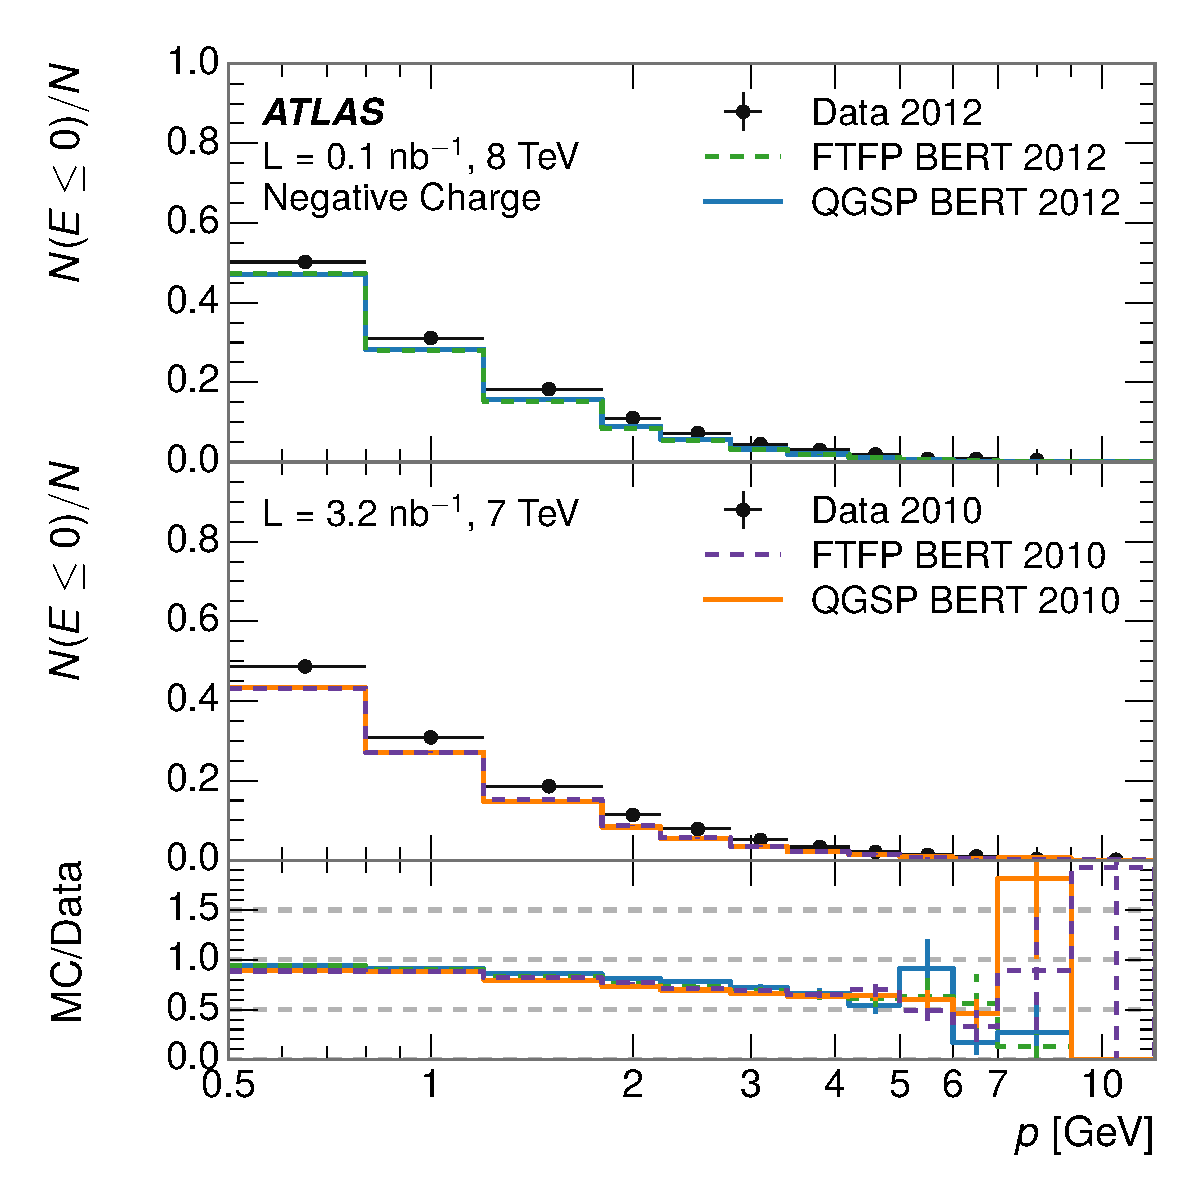
\includegraphics[width=0.48\textwidth]{figures/dvmc_ezero_layer01_calib01_eta01_q01_nc00_trt00.pdf}
}
\\
\subfloat[]{
  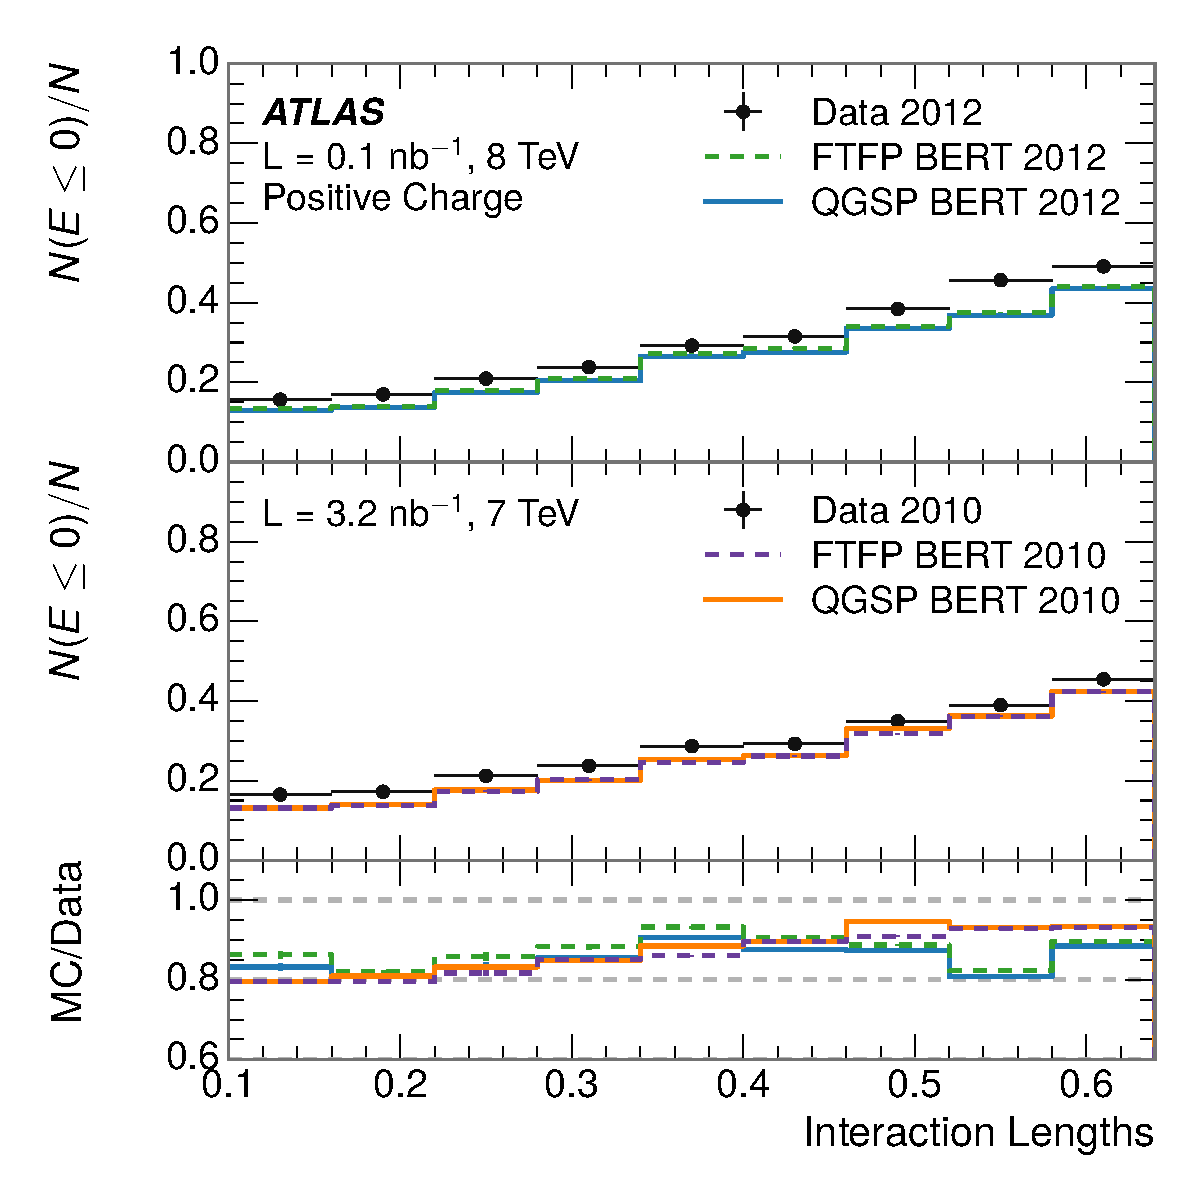
\includegraphics[width=0.48\textwidth]{figures/ezero_intlen_q02.pdf}
}
~
\subfloat[]{
  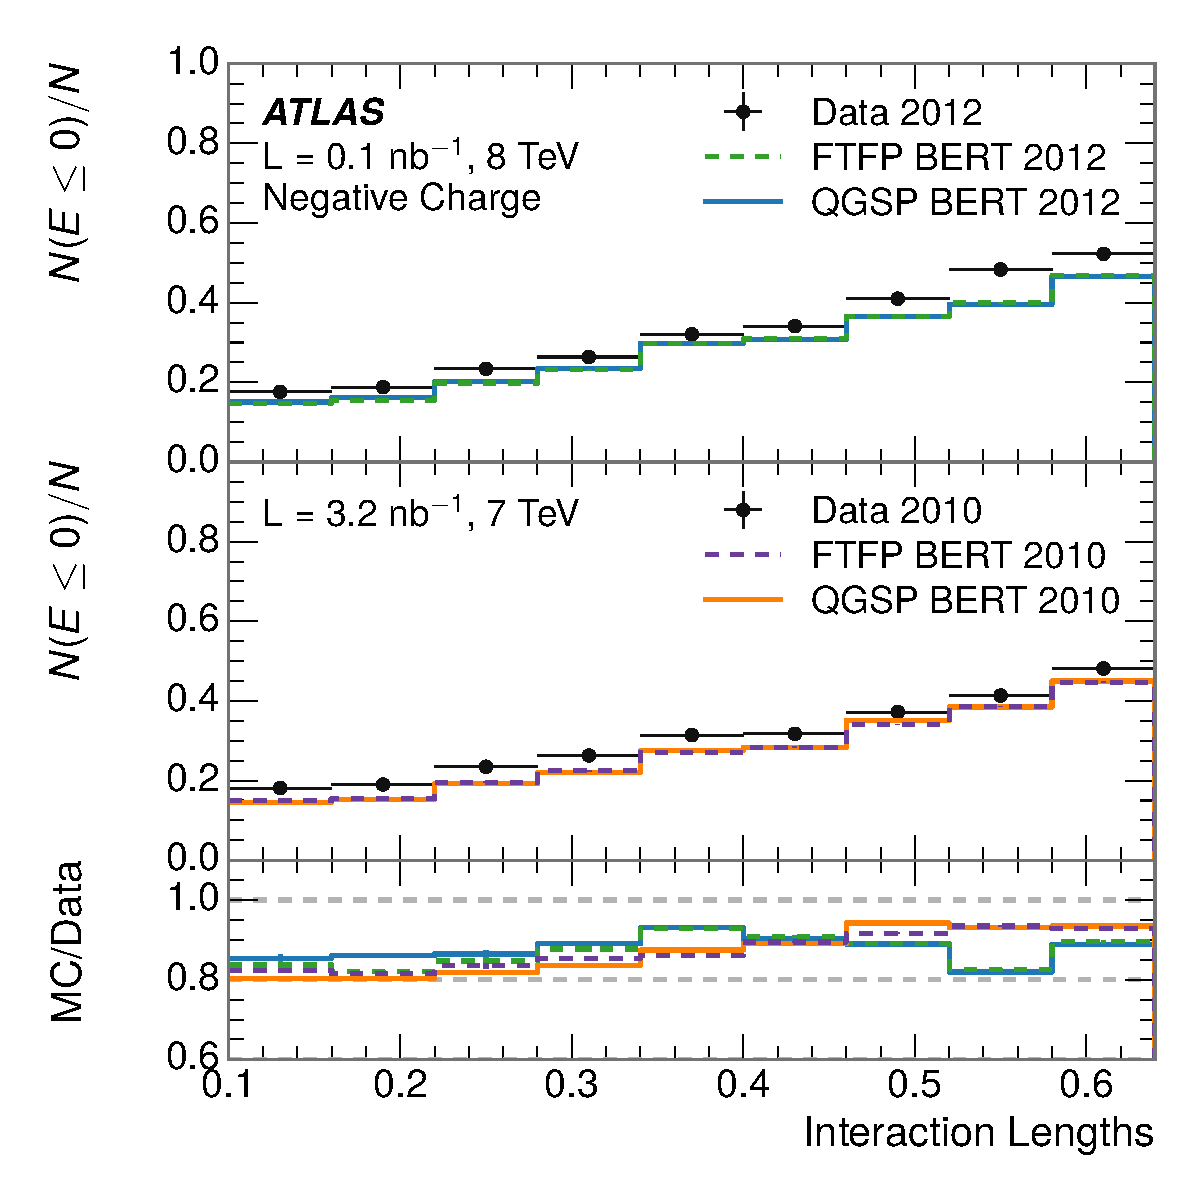
\includegraphics[width=0.48\textwidth]{figures/ezero_intlen_q01.pdf}
}
\caption{The fraction of tracks as a function (a, b) of momentum, (c, d) of interaction lengths with $E \leq 0$ for tracks with positive (on the left) and negative (on the right) charge.}
\label{fig:zerofracincl}
\end{figure}


\subsection{Neutral Background Subtraction}
\label{sec:neutral_bg}

The isolation requirement on hadrons is only effective in remove energy contribution from nearby charged particles. 
Nearby neutral particles, predominantly photons from \piz decays, also add their energy to the calorimeter clusters, but mostly in the electromagnetic calorimeter. 
It is possible to measure this contribution, on average, using late-showering hadrons that minimally ionize in the electromagnetic calorimeter. 
Such particles are selected by requiring that they deposit less than 1.1 \GeV in the EM calorimeter within a cone of $\Delta R < 0.1$ around the track. 
To ensure that these particles are well measured, they are additionally required to deposit between 40\% and 90\% of their energy in the hadronic calorimeter within the same cone. 

These particle provide a clean sample to measure the nearby neutral background because they do not deposit energy in the area immediately surrounding them in the EM calorimeter, as shown in Figure~\ref{fig:eoverp_cartoon}.
So, the energy deposits in the region $0.1 < \Delta R < 0.2$ can be attributed to neutral particles alone.
To estimate the contribution to the whole cone considered for the response measurement, that energy is scaled by a geometric factor of 4/3. 
This quantity, \epbg, measured in aggregate over a number of particles, gives the contribution to \epav from neutral particles in the EM calorimeter. 
Similar techniques were used in the individual layers of the hadronic calorimeters to show that the background from neutrals is negligable in those layers~\cite{PERF-2011-05}. 

The distribution of this background estimate is shown in Figure~\ref{fig:eoverp_background}. 
Although the simulation captures the overall trend, it significantly overestimates the neutral contribution for tracks with momentum between 2 and 8 \GeV.
This effect was also seen in the tails of the \ep distributions in Figure~\ref{fig:eoverp}.
This difference is likely due to the modelling of coherent neutral particle radiation in \texttt{Pythia8}, as the discrepancy does not depend on $\eta$ and thus is unlikely to be a mismodelling of the detector.
This difference can be subtracted however, to form $\epcor \equiv \epav - \epbg$, which measures the average calorimeter response without the contamination of neutral particles.

\begin{figure}[htbp]
\centering
\subfloat[]{
  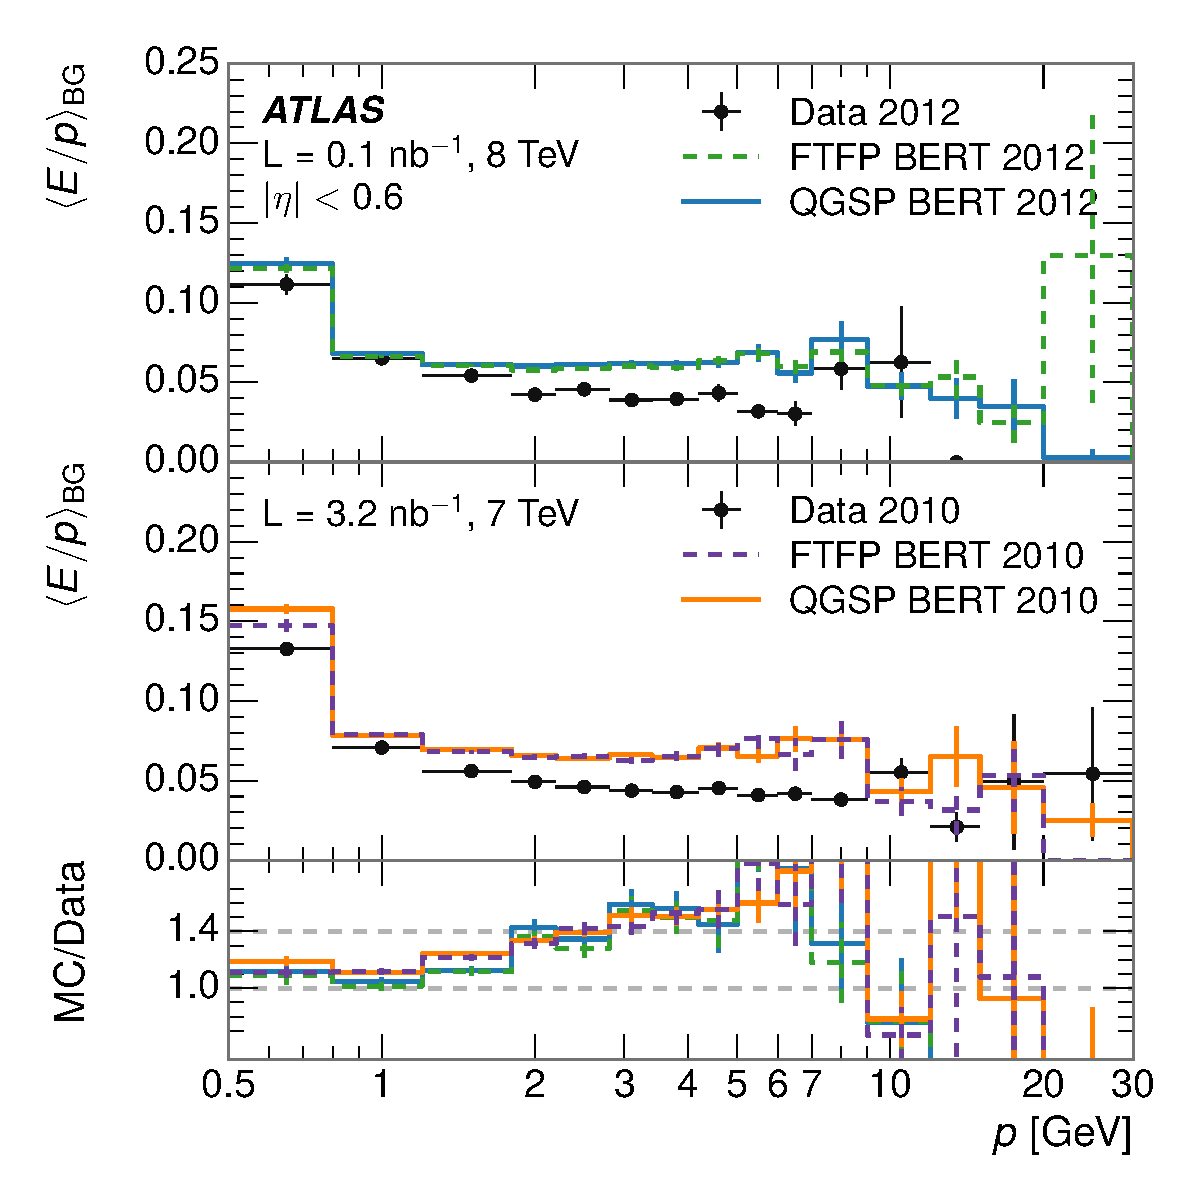
\includegraphics[width=0.48\textwidth]{figures/dvmc_epbg_layer01_calib01_eta01_q00_nc00_trt02.pdf}
}
~
\subfloat[]{
  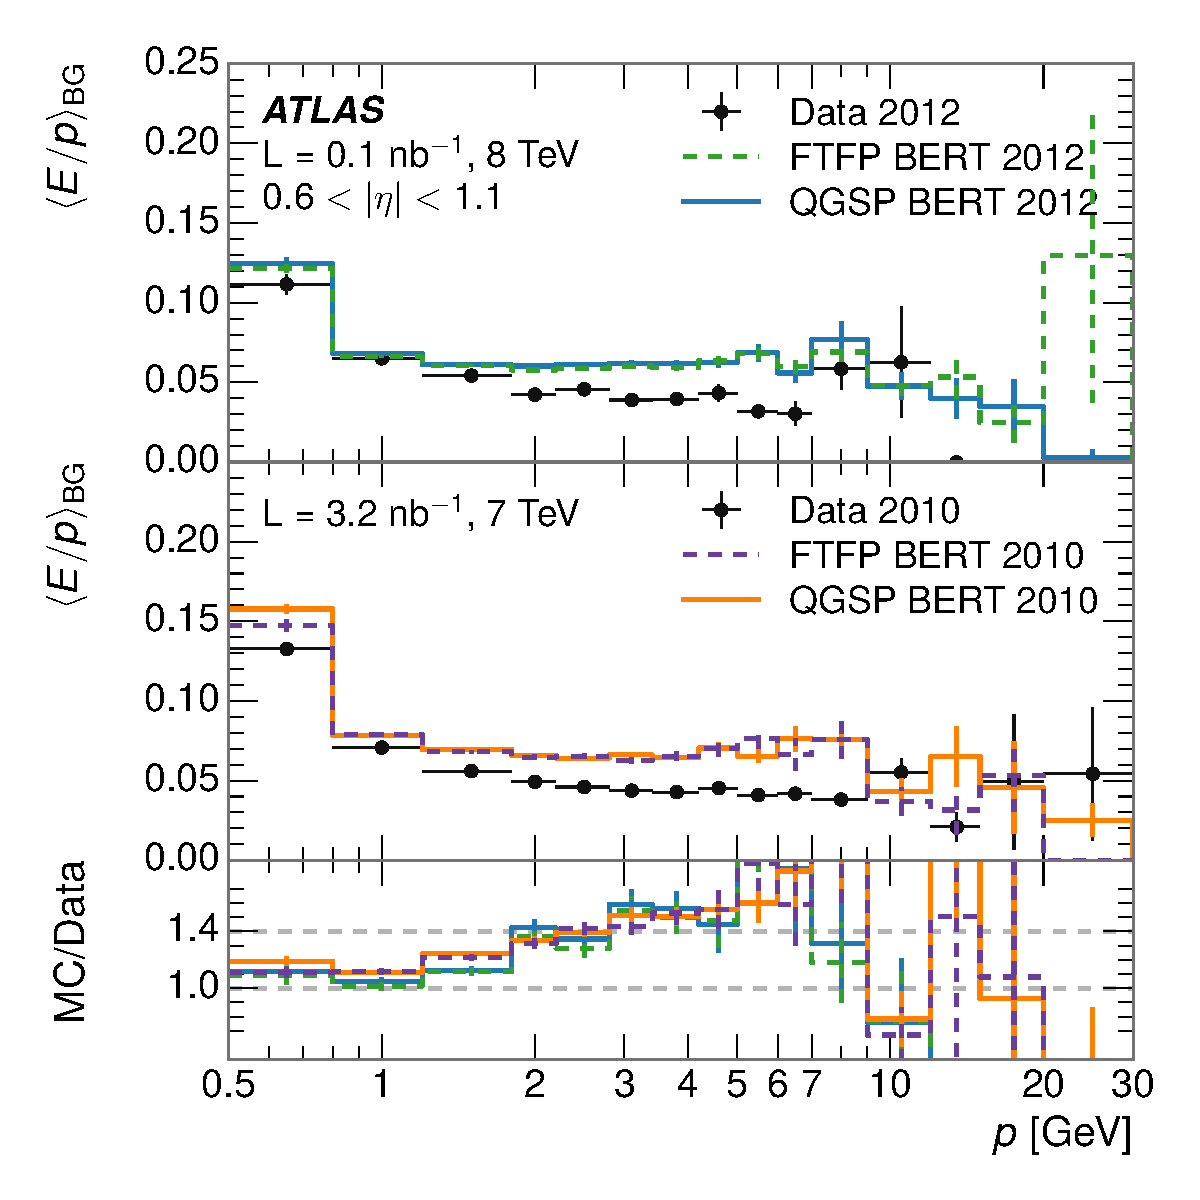
\includegraphics[width=0.48\textwidth]{figures/dvmc_epbg_layer01_calib01_eta02_q00_nc00_trt02.pdf}
}
\\
\subfloat[]{
  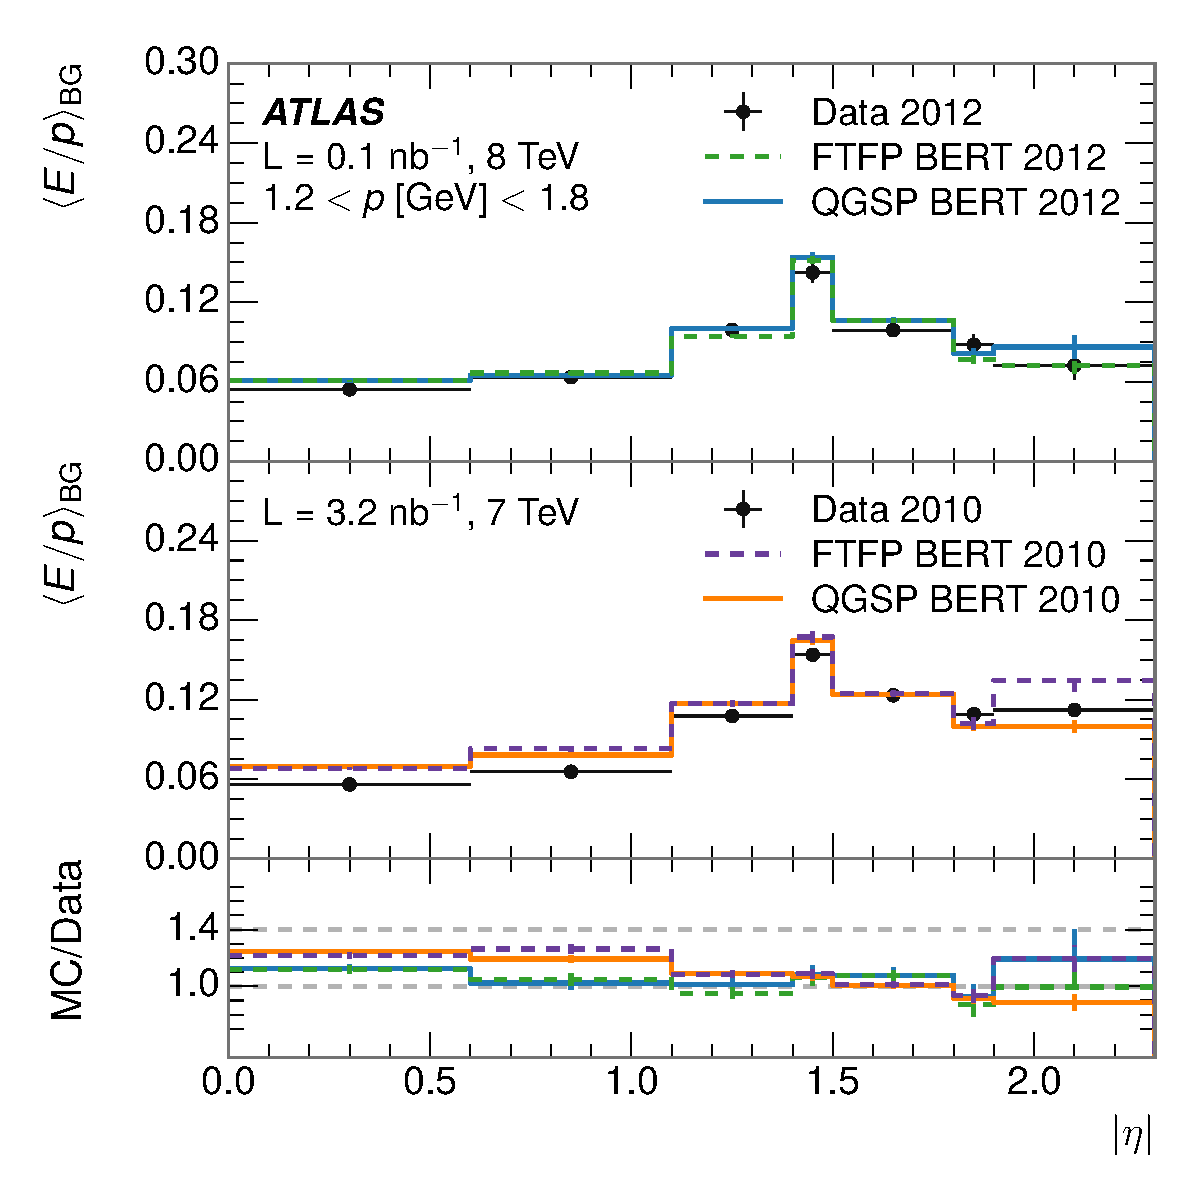
\includegraphics[width=0.48\textwidth]{figures/dvmc_epbg_layer01_calib01_p03_q00_nc00_trt02.pdf}
}
~
\subfloat[]{
  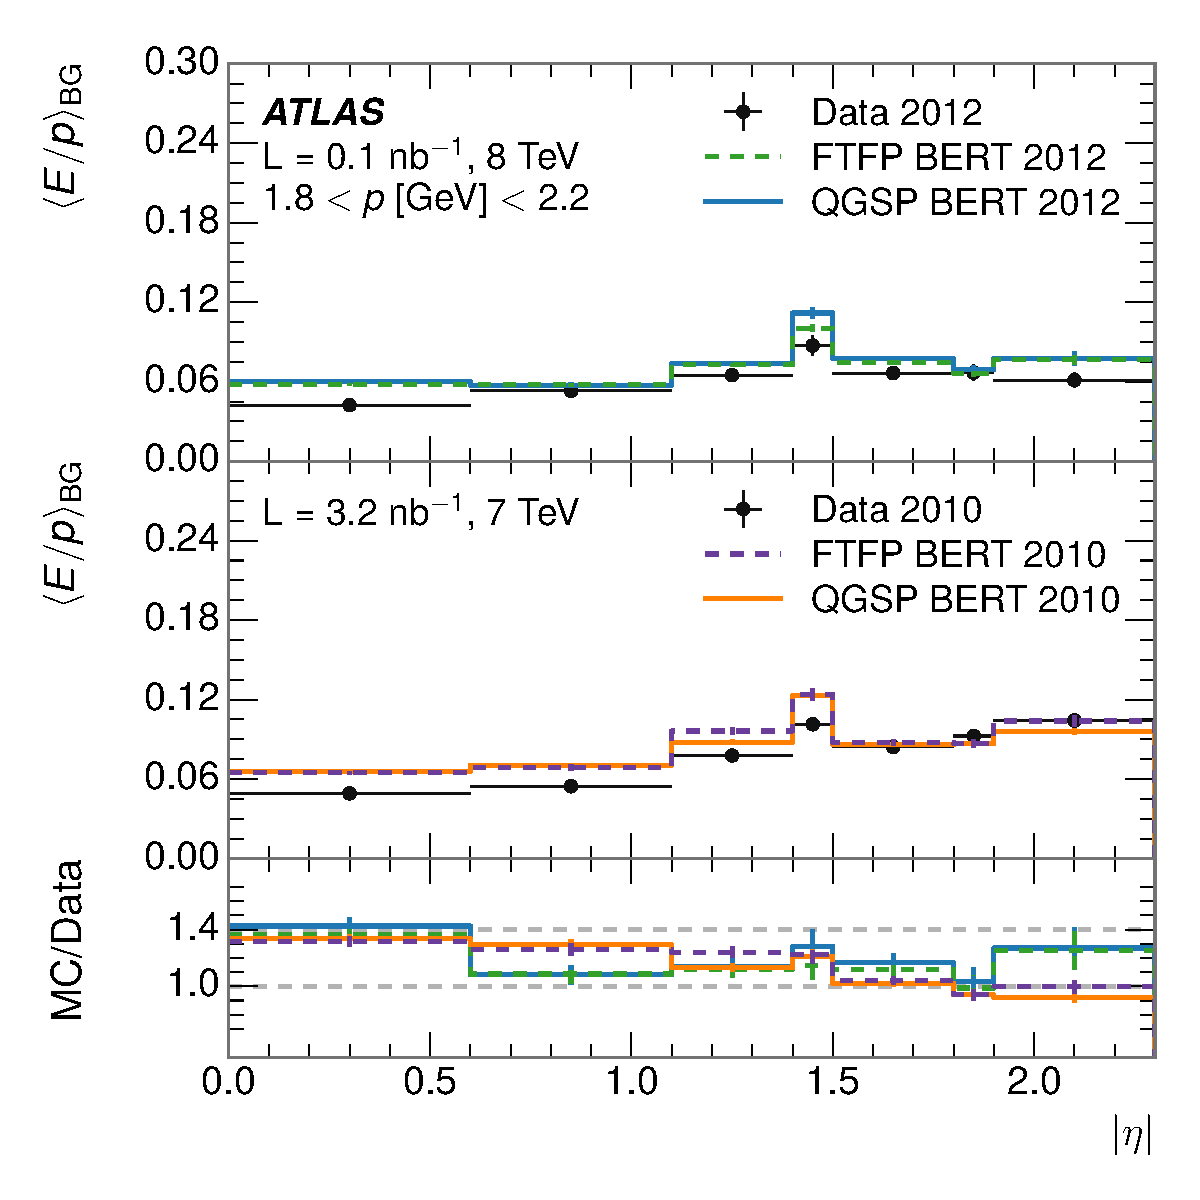
\includegraphics[width=0.48\textwidth]{figures/dvmc_epbg_layer01_calib01_p04_q00_nc00_trt02.pdf}
}
\caption{\epbg as a function of the track momentum and (a) $|\eta| < 0.6$, (b) $0.6 < |\eta| < 1.1$, and as a function of the track pseudorapidity and (c) $1.2 < p / \GeV < 1.8$, (d) $1.8 < p / \GeV < 2.2$.}
\label{fig:eoverp_background}
\end{figure}

\subsection{Corrected Response}
\label{sec:response}

\subsubsection{Clustering}
\label{sec:clustering}

\subsubsection{Additional Studies}
\label{sec:additional}

% ----------------------------------------

\section{Identified Particle Response}
\label{sec:identified}

% ----------------------------------------
